Für den praktischen Anteil dieser Arbeit wird auf Grundlage der gewonnenen Erkenntnisse aus Sektion 3 ein Prototyp angefertigt. Es wird also auf die Hypothesen zurückgegriffen, welche durch die Interviews und Umfragen erarbeitet und überprüft wurden. Außerdem wird anhand eines geeigneten Beispiels der Natur eine Thematik Stück für Stück untersucht und in Mechaniken transformiert. Konkret werden in Folgendem die Vorgänge innerhalb einer Bienenkolonie genauer beleuchtet, und erörtert, welche Elemente sich für ein Resource Management Game eignen.

\subsubsection{Thematik}
Für den Prototypen bedarf es einer Thematik beziehungsweise einer Idee für das Gesamtkonzept. Dafür wurde die Idee einer \textit{Bienenkolonie} für interessant befunden. Bienen und deren Kolonien sind aus vielerlei Hinsicht geeignet als Thematik für den Prototyp, darunter der Fakt, dass Bienen bekannt dafür sind, Honig zu produzieren, wobei Honig eine konkrete Ressource darstellt. Im Kontext eines Resource Management Games und mit Rücksicht auf das zuvor untersuchte Spiel \textit{RimWorld} eignet sich jedoch am besten eine ganz spezifische Art der Bienen, die \textit{Honigbiene}, genauer gesagt die \textit{Westliche Honigbiene} (lat. \textit{apis mellifera}) \cite*[]{bees:name}. Grund dafür ist die Verhaltensweise von Honigbienen, da diese, anders als nahe Verwandte, stärker dazu tendieren, in Kolonien zu leben. Hummeln beispielsweise formen zwar auch Kolonien, aber deutlich kleinere und kürzer lebende. Die meisten Arten der Wildbienen jedoch sind tendenziell Einzelgänger. Eine weibliche Wildbiene legt ein Nest und versorgt ihren Nachwuchs mit Pollen und Nektar \cite*[]{bees:wild}. Somit bietet die Gattung der Honigbiene einige Vorgänge, welche sich in ein Colony Management Game umsetzen lassen. Dazu werden im Folgenden interessante Vorgänge und Eigenschaften der Gattung der Honigbiene genauer untersucht.

\newparagraph{Nahrung}
Eine Honigbiene ernährt sich primär von \textit{Nektar}, welchen sie von Blumen sammelt. Dieser Nektar ist zuckerhaltiger Saft, welcher von den Pflanzen ausgeschieden wird, um damit Insekten verschiedener Arten anzulocken. Dabei sind Sonnenblumen, Obstblüten, Löwenzahn und Raps besonders gute Nektarquellen \cite*[]{bees:food}. Eine weitere Möglichkeit um an energiereichen Zucker zu gelangen ist der sogenannte \textit{Honigtau}, welcher von einigen Insekten, darunter Blatt- und Schildläusen, ausgeschieden wird. Aus diesen beiden zuckerhaltigen Säften können die Bienen den \textit{Honig} produzieren, welcher ebenfalls als Nahrungsquelle dient, aber vor allem über die Wintermonate besonders wichtig ist, da Honig sehr lange haltbar ist \cite*[]{bees:honeywinter}. Der durch Honigtau produzierte Honig wird von Imkern als \textit{Waldhonig} gekennzeichnet \cite*[]{bees:food}. Saugt eine Biene den Nektar einer Blüte auf, gelangt dieser in den \textit{Honigmagen}. Dort kommt er in Kontakt mit verschiedenen Enzymen, welche den Nektar in \textit{Glukose} (Traubenzucker) und \textit{Fruktose} (Fruchtzucker) \cite*[]{bees:glucosefructose} aufspalten. Diesen biochemisch veränderten Nektar gibt die \textit{Sammelbiene} im Bienenstock an die sich dort befindlichen \textit{Arbeitsbienen} durch Auswürgen weiter, welche den Nektar erneut aufnehmen und auswürgen. Mit jedem dieser Prozesse wird der Nektar viskoser, wodurch allmählich Honig entsteht \cite*[]{bees:nectartohoney}.

Neben dem Nektar, dem Honigtau und dem Honig, welche primär als Quellen für Kohlenhydrate dienen, benötigen Bienen außerdem noch Quellen für Fette und Proteine. Dafür werden \textit{Pollen} verwendet, wobei Pollen die männlichen Geschlechtszellen einer Samenpflanze sind. Da die Samenpflanze mehr Pollen produziert, als für die Fortpflanzung nötig, können diese ohne Probleme von den Sammelbienen aufgenommen werden \cite*[]{bees:honeywinter}. Die Pollen werden in \textit{Pollenpaketen} aufbewahrt (vgl. \autoref{image:pollenpaket}), wobei Teile der aufgesammelten Pollen nicht in diesen Pollenpaketen landen, sondern an den Hinterbeinen haften bleiben. Besucht diese Sammelbiene nun eine weitere Blüte, werden diese Pollen abgestreift und der Fortpflanzungsmechanismus der Samenpflanze profitiert. Besonders pollenreiche Quellen sind dabei Obstbäume, Mohn, Mais, Klee und Raps \cite*[]{bees:honeywinter}.

\begin{figure}
    \begin{center}
        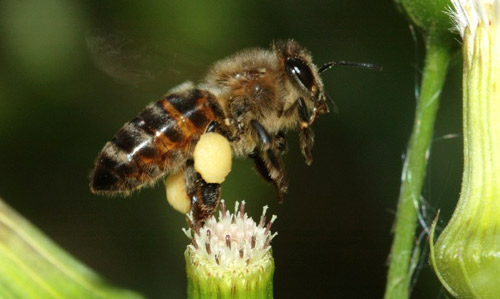
\includegraphics[width=300px]{0.bilder/pollenpaket.jpg}
    \end{center}
    \caption{Pollenpakete einer Honigbiene (\cite{bees:name})} \label{image:pollenpaket}
\end{figure}

Die letzte wichtige Ressource, welche Bienen für ihr Überleben benötigen, ist Wasser. Dieses kann von Flüssen oder Seen bezogen werden, wobei diese Quellen nicht mehr als 500 Meter weit vom Stock entfernt sein sollten. Erhalten Bienen nicht genug Wasser, können diese unter Verstopfungen leiden, was für das Überleben gefährlich sein kann \cite*[]{bees:honeywinter, bees:food}.

Es lassen sich somit wichtige Ressourcen identifizieren: \textit{Nektar, Honigtau, Honig, Pollen} und \textit{Wasser}. Außerdem ist die Aufteilung zwischen \textit{Sammel-} und \textit{Arbeitsbiene} eine mögliche Mechanik. Die Umwandlung von Nektar und Honigtau zu Honig könnte ebenfalls eine Mechanik darstellen, wie auch die naturgegebenen Quellen für Nektar, Honigtau und Pollen.